\begin{center}
	\begin{circuitfig}[H]
		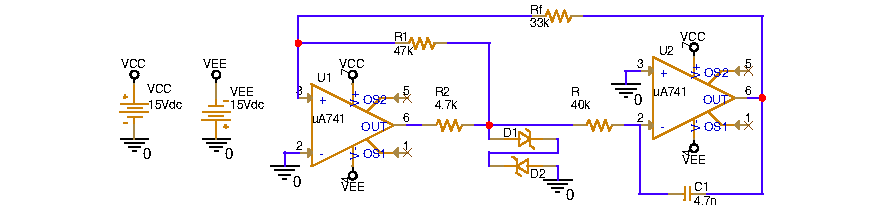
\includegraphics[width=15cm]{spice_01/schematic.pdf}
		\caption{Κύκλωμα προσομοίωσης για το PSpice.}
		\label{circ:spice:1_schematic}
	\end{circuitfig}
\end{center}

Οι προσομοιώσεις έγιναν με το κύκλωμα \ref{circ:spice:1_schematic}. Οι δίοδοι Zener\footnote{Χρησιμοποιήθηκαν δεδομένα από data sheet της διόδου 1N5236B του εμπορίου.}, D1 και D2, δημιουργήθηκαν χρήσει του \textsl{PSpice Modeling Application}. Η τάση Zener των διόδων ορίστηκε $V_Z=7.5\unit{\volt}$ και ο θερμοκρασιακός συντελεστής ορίσθηκε στο $0.058\displaystyle{\sfrac{\%}{\unit{\celsius}}}$.


\begin{chart}[H]
	\begin{center}
		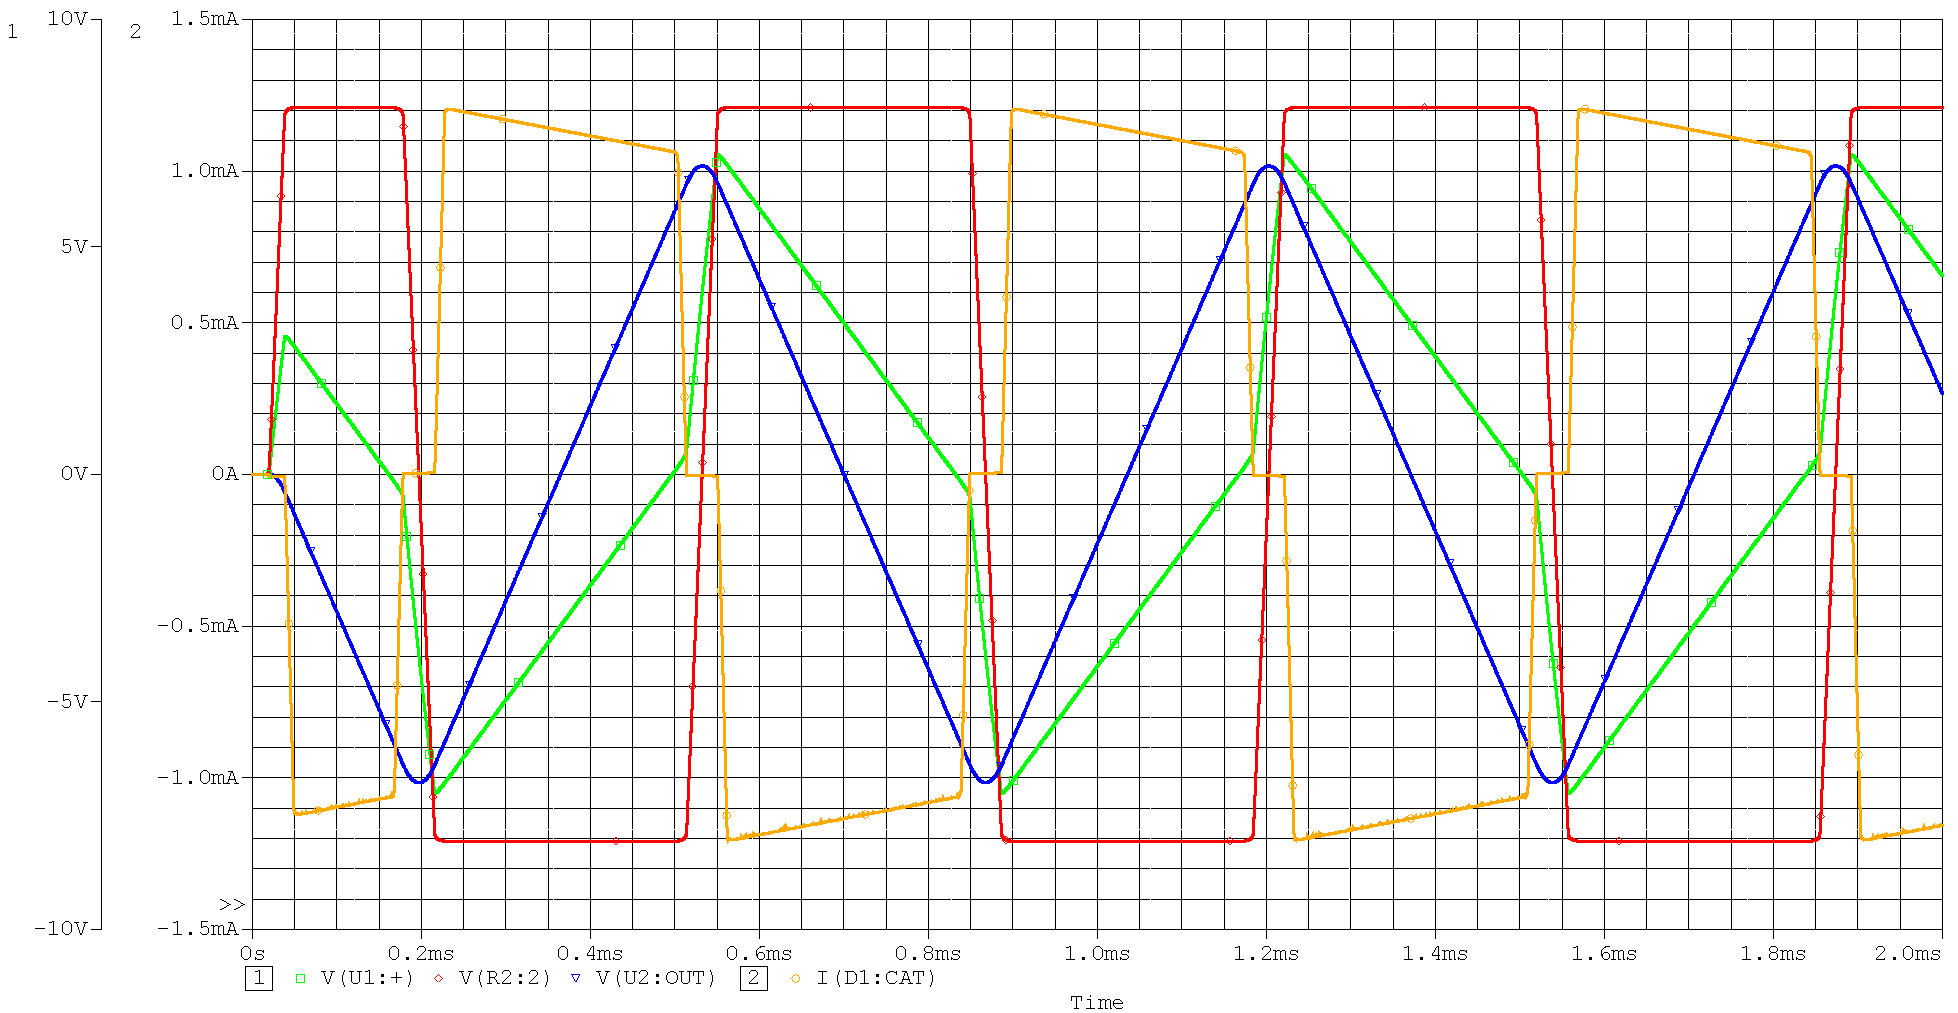
\includegraphics[width=15cm]{spice_01/q4cropped.pdf}
		\caption{Οι τάσεις $V_1$ (πράσινη κυματομορφή), $V_2$ (κόκκινη κυματομορφή) και $V_{\mathrm{out}}$ (μπλε κυμματομορή) και το ρεύμα $I_Z$ (πορτοκαλί κυματομορφή).}
		\label{plot:ask1:q4}
	\end{center}
\end{chart}

Οι περίοδοι των κυματομορφών βρέθηκαν με τη βοήθεια της συνάρτησης \texttt{Period()}. Τα αποτελεσματα φαίνονται στον πίνακα \ref{table:ask1:q4:periods}.

\begin{table}[h]
	\begin{center}
		\begin{tabular}{|c|c|c|}
			\hline
			\textbf{Σήμα}      & \textbf{Περίοδος}               & \textbf{Μέγιστη τιμή}        \\
			\hline
			\hline
			$V_1$              & $479.05597\unit{\micro\second}$ & $7.0205\unit{\volt}$         \\\hline
			$V_2$              & $670.70736\unit{\micro\second}$ & $8.0655\unit{\volt}$         \\\hline
			$V_{\mathrm{out}}$ & $670.70736\unit{\micro\second}$ & $6.7789\unit{\volt}$         \\\hline
			$I_Z$              & $670.70871\unit{\micro\second}$ & $1.2045\unit{\milli\ampere}$ \\\hline
		\end{tabular}
		\caption{Περίοδοι κυματομορφών του διαγράμματος \ref{plot:ask1:q4}.}
		\label{table:ask1:q4:periods}
	\end{center}
\end{table}